\documentclass[a4paper,titlepage]{article}
\usepackage[top=1in, bottom=1.25in, left=1.25in, right=1.25in]{geometry}

\parskip=10pt

\usepackage[scaled]{beramono}
\usepackage[T1]{fontenc}

\usepackage{amsmath}

\usepackage{listings}
\lstset{basicstyle=\footnotesize\ttfamily,tabsize=4,breaklines,frame=single, moredelim=[is][\underbar]{__}{__}}

\usepackage{graphicx}
\usepackage{tikz}
\usepackage{float}
\usepackage{booktabs}

\def\checkmark{\tikz\fill[scale=0.4](0,.35) -- (.25,0) -- (1,.7) -- (.25,.15) -- cycle;} 
\def\scalecheck{\resizebox{\widthof{\checkmark}*\ratio{\widthof{x}}{\widthof{\normalsize x}}}{!}{\checkmark}}

\renewcommand{\figurename}{Gambar}
\renewcommand{\refname}{Referensi}

\begin{document}

	\title{Laporan Tugas Kecil III - Penyelesaian \textit{Travelling Salesperson Problem} dengan \textit{Branch and Bound} \\ IF2211 Strategi Algoritma}
	\author{Jonathan Christopher / 13515001 / K-01}
	\maketitle

	\section{Deskripsi Persoalan}

		Persoalan yang harus diselesaikan dalam tugas ini adalah membuat sebuah program yang dapat menyelesaikan persoalan \textit{travelling salesperson problem} (TSP), yaitu mencari tur lengkap terpendek dari sebuah graf, menggunakan algoritma \textit{branch and bound}. Tur lengkap adalah sebuah rute yang mendatangi setiap simpul tepat satu kali, kemudian kembali ke simpul awal. Program harus menggunakan dua pendekatana yang berbeda, yaitu \textit{branch and bound} dengan \textit{bounding function} berupa \textit{reduced cost matrix} atau bobot tur lengkap. Program juga harus bisa membaca masukan dari sebuah \textit{file} teks, menampilkan graf yang dicari tur lengkap terpendeknya beserta dengan solusi dan bobot tur lengkap terpendeknya, menampilkan jumlah simpul yang dibangkitkan, serta menampilkan waktu yang dibutuhkan untuk perhitungan.

	\section{Penyelesaian Persoalan}

		Penulis pada mengimplementasikan solusi menggunakan Python 2.7. Penulis menggunakan \textit{library} NumPy (http://www.numpy.org, NumPy License) yang menyediakan representasi dan operasi matriks yang lebih efisien. Untuk penggambaran graf, penulis menggunakan \textit{library} GraphViz (http://www.graphviz.org, Eclipse Public License v1.0).

		\begin{table}[H]
			\centering
			\begin{tabular}{@{}lcc@{}}
				\toprule
				Poin 																			 & Ya 		  & Tidak \\ \midrule
				Program berhasil dikompilasi 													 & \checkmark &       \\
				Program berhasil di-\textit{run}												 & \checkmark &       \\
				Program dapat membaca masukan dan menuliskan keluaran 							 & \checkmark &       \\
				Solusi TSP benar dengan fungsi pembatas \textit{reduced cost matrix}		 	 & \checkmark &       \\
				Solusi TSP benar untuk fungsi pembatas bobot tur lengkap 						 & \checkmark &       \\
				\bottomrule
			\end{tabular}
			\caption{Tabel poin-poin yang berhasil diimplementasi}
			\label{tab:implementasi}
		\end{table}

	\section{\textit{Source Code}}

		\subsection{tsp-bb.py}
		\lstinputlisting[language=Python]{../tsp-bb.py}

		\subsection{branchandbound.py}
		\lstinputlisting[language=Python]{../branchandbound.py}

	\section{Contoh Interaksi dengan Program}

		Berikut adalah contoh-contoh interaksi pengguna dengan program. Program membaca input dari \textit{file} teks yang diberikan sebagai argumen pertama program.

		\noindent Penulis menguji program pada sistem dengan spesifikasi sebagai berikut:
		\begin{itemize}
			\item Prosesor Intel Core i7 4720HQ 3,6 GHz
			\item RAM 4GB DDR3
			\item Sistem operasi Windows 10 64-bit
			\item Python 2.7.11
		\end{itemize}

		\subsection{Contoh Masukan/Keluaran 1}

		\lstinputlisting{../1.in}

		\begin{lstlisting}
Travelling Salesman Problem Solver
13515001 (K01) - Jonathan Christopher
IF2211 Strategi Algoritma
-------------------------------------

Reading input graph from file...
Using reduced cost matrix bounding function:
Starting solver...

Shortest cycle distance: 171
Path: [1, 8, 3, 2, 6, 4, 7, 5, 1]
Nodes generated: 46
Nodes visited: 16
Execution time: 0.0169999599457 seconds.
		\end{lstlisting}

		\begin{figure}[H]
		    \centering
		    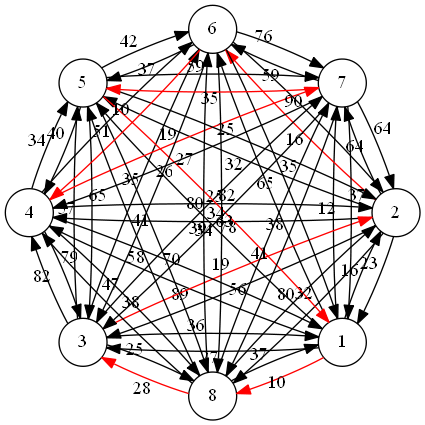
\includegraphics[width=0.6\textwidth]{1.png}
		    \caption{Solusi \textit{travelling salesperson problem} menggunakan fungsi pembatas \textit{reduced cost matrix} untuk masukan 1}
		    \label{fig:hasileksekusi1}
		\end{figure}

		\subsection{Contoh Masukan/Keluaran 2}

		\lstinputlisting{../2.in}

		\begin{lstlisting}
Travelling Salesman Problem Solver
13515001 (K01) - Jonathan Christopher
IF2211 Strategi Algoritma
-------------------------------------

Reading input graph from file...
Using reduced cost matrix bounding function:
Starting solver...

Shortest cycle distance: 451
Path: [1, 2, 3, 4, 5, 6, 7, 8, 9, 10, 1]
Nodes generated: 46
Nodes visited: 11
Execution time: 0.0310001373291 seconds.
		\end{lstlisting}

		\begin{figure}[H]
		    \centering
		    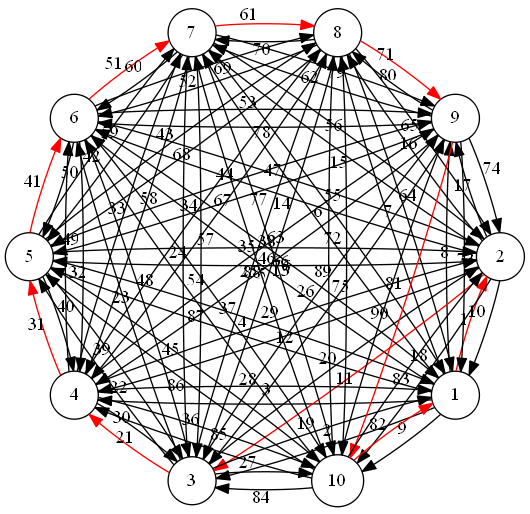
\includegraphics[width=0.7\textwidth]{2.png}
		    \caption{Solusi \textit{travelling salesperson problem} menggunakan fungsi pembatas \textit{reduced cost matrix} untuk masukan 2}
		    \label{fig:hasileksekusi2}
		\end{figure}

		\subsection{Contoh Masukan/Keluaran 3}

		\lstinputlisting{../3.in}

		\begin{lstlisting}
Travelling Salesman Problem Solver
13515001 (K01) - Jonathan Christopher
IF2211 Strategi Algoritma
-------------------------------------

Reading input graph from file...
Using complete tour cost bounding function
Starting solver...

Shortest cycle distance: 183
Path: [1, 8, 3, 6, 2, 5, 4, 7, 1]
Nodes generated: 65
Nodes visited: 17
Execution time: 0.0220000743866 seconds.
		\end{lstlisting}

		\begin{figure}[H]
		    \centering
		    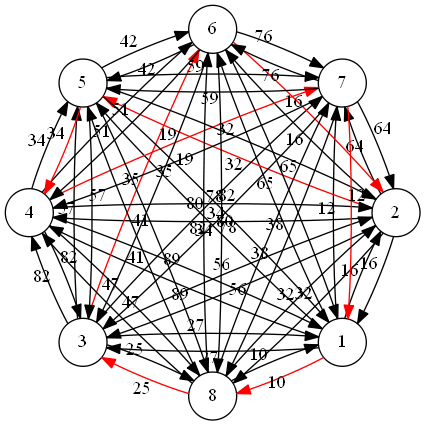
\includegraphics[width=0.6\textwidth]{3.png}
		    \caption{Solusi \textit{travelling salesperson problem} menggunakan fungsi pembatas bobot tur lengkap untuk masukan 3}
		    \label{fig:hasileksekusi3}
		\end{figure}

		\subsection{Contoh Masukan/Keluaran 4}

		\lstinputlisting{../4.in}

		\begin{lstlisting}
Travelling Salesman Problem Solver
13515001 (K01) - Jonathan Christopher
IF2211 Strategi Algoritma
-------------------------------------

Reading input graph from file...
Using complete tour cost bounding function
Starting solver...

Shortest cycle distance: 250
Path: [1, 6, 3, 7, 4, 8, 2, 9, 5, 10, 1]
Nodes generated: 250713
Nodes visited: 87203
Execution time: 133.770999908 seconds.
		\end{lstlisting}

		\begin{figure}[H]
		    \centering
		    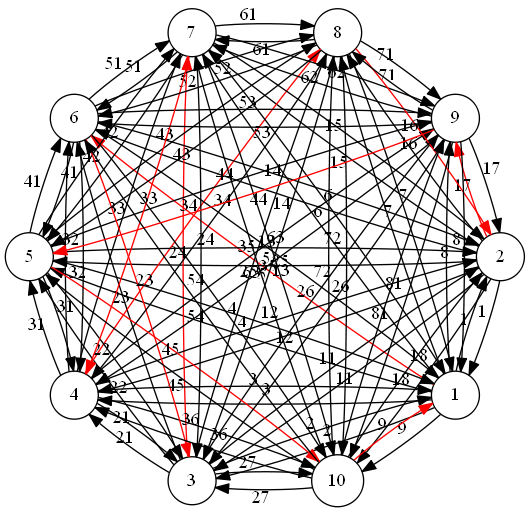
\includegraphics[width=0.7\textwidth]{4.png}
		    \caption{Solusi \textit{travelling salesperson problem} menggunakan fungsi pembatas bobot tur lengkap untuk masukan 4}
		    \label{fig:hasileksekusi4}
		\end{figure}
		
\end{document}